\documentclass[hidelinks,12pt]{article}
\usepackage{graphicx}
\usepackage{layout}
\usepackage{amsmath, amssymb}
\usepackage{hyperref}
\usepackage{float}
\usepackage{fancyhdr}
\usepackage{titlesec}
\usepackage[dvipsnames]{xcolor}
\usepackage{lipsum}
\usepackage{cleveref}
\usepackage[a4paper,left=3cm,right=2cm,top=2.5cm,bottom=2.5cm]{geometry}
\usepackage{overpic}
\usepackage{booktabs}
\usepackage{subcaption}
\usepackage{titlesec}
\usepackage{caption}
\usepackage{lipsum}
\usepackage{enumitem}

\pagestyle{fancy}
\fancyhf{}
% \renewcommand{\headrulewidth}{0pt}
\cfoot{\thepage}

\setlength{\parindent}{0pt}

\graphicspath{ {./figs/} }

\author{M.M. Roshani}

\begin{document}
	\begin{titlepage}
		\begin{center}
			\begin{figure}
				\vspace{-1.0cm}
				\centering
				
\includegraphics[scale=0.35]{SUT_logo}
			\end{figure}
			\mbox{}\\[2.0cm]
			\textsc{\Huge \textbf{Signals and Systems Project}}\\[1.0cm]
			\textsc{\LARGE Phase 1}\\[1.5cm]
			\textsc{\LARGE Instructor: Prof. Hamid Aghajan}\\[1cm]
			\textsc{\LARGE Sharif University of Technology}\\[1.0cm]
			\rule{\linewidth}{0.5mm} \\
			{\large \bf {\fontfamily{cmss}\selectfont Analysis of Phase-Amplitude Coupling during Olfactory Stimulation \\ \medskip as a Biomarker for Alzheimer's Disease in EEG Signals}}\\[0.2cm]
			\rule{\linewidth}{0.5mm} \\
			\vfill
			{\Large M.M. Roshani}
		\end{center}
	\end{titlepage}
	
	\tableofcontents
	\newpage
	
	
	Since we have three patients and preprocessing differs for each one slightly, we discuss them separately. The preprocessing is based on a \href{https://sccn.ucsd.edu/wiki/Makoto's_preprocessing_pipeline#Further_optimizing_the_preprocessing_order.3F_.2802.2F28.2F2020_updated.29}{\textcolor{Cyan}{a document}} by Makoto.
	
	\section{Healthy Control}
	\subsection{Load EEG Data and Set Channel Locations}
	After opening EEGLAB, we import our data from the following menu:
	
	File > Import data > Using EEGLAB functions and plugins > From ASCII/float file or MATLAB array.

		\begin{figure}[h!]
			\centering
			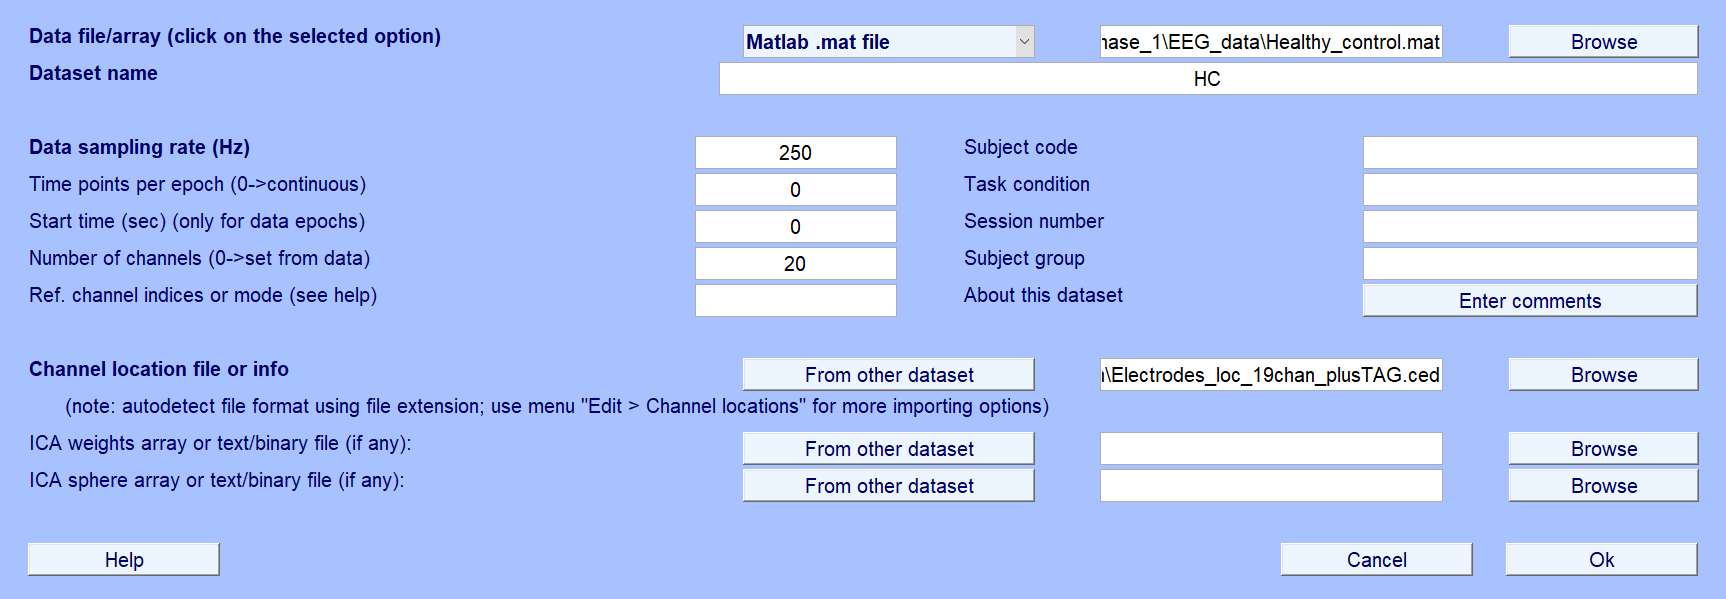
\includegraphics[width=0.9\textwidth]{1}
			\caption{Loading HC dataset}
		\end{figure}
		
	Based on the information we have about the sampling process, we set the sampling rate to 250Hz and the number of channels to 20. The rest of the fields will be filled based on the dataset itself. Then we add our channel location file and the loading step is complete.
	
	
	
	\subsection{Import Event Information}
	We import event information and then remove the associated channel (20).
	
	File > Import event info > From data channel.
	
		\begin{figure}[h!]
			\centering
			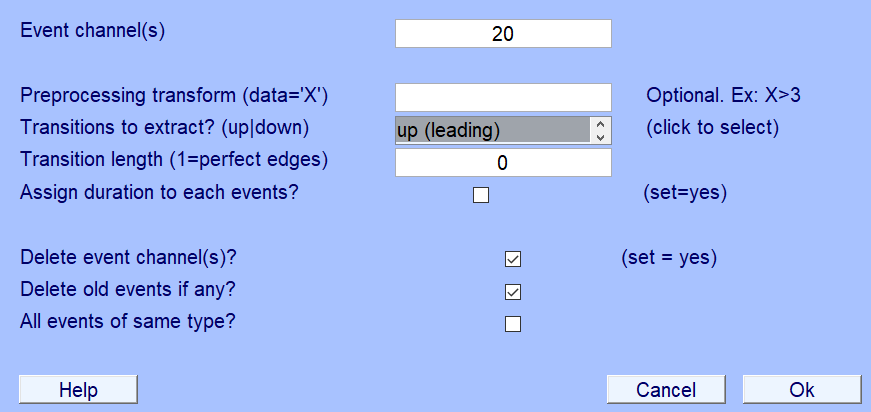
\includegraphics[width=0.6\textwidth]{2}
			\caption{Importing event information}
		\end{figure}
		
	
	\newpage
	
	\subsection{Filtering}
	We apply a bandpass filter (1–90 Hz) to remove slow drifts and high-frequency noise. Then, a notch filter (48–52 Hz) is applied to eliminate line noise.
	
	Tools > Filter the data > Basic FIR filter.
	
	\begin{figure}[!h]
		\centering
		\begin{subfigure}{0.45\textwidth}
			\centering
			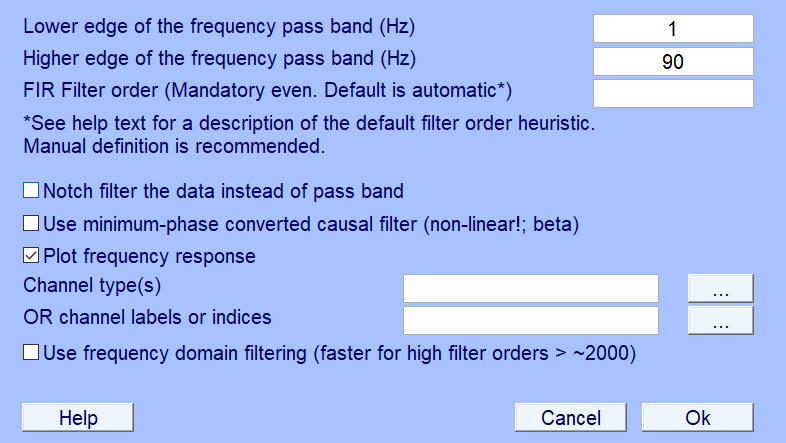
\includegraphics[width=\linewidth]{3}
			\vspace{0.5cm}
		\end{subfigure}
		\hfill
		\begin{subfigure}{0.45\textwidth}
			\centering
			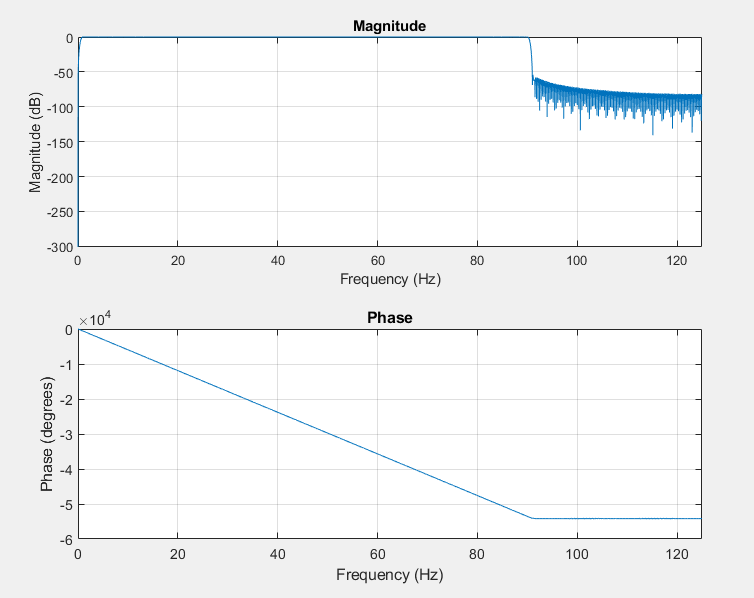
\includegraphics[width=\linewidth]{4}
		\end{subfigure}
		\caption{Bandpass filter}
	\end{figure}
	
	\begin{figure}[!h]
		\centering
		\begin{subfigure}{0.45\textwidth}
			\centering
			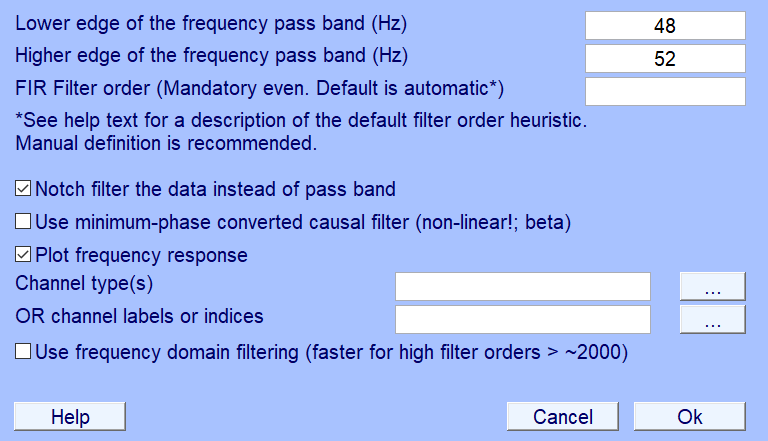
\includegraphics[width=\linewidth]{5}
			\vspace{0.3cm}
		\end{subfigure}
		\hfill
		\begin{subfigure}{0.45\textwidth}
			\centering
			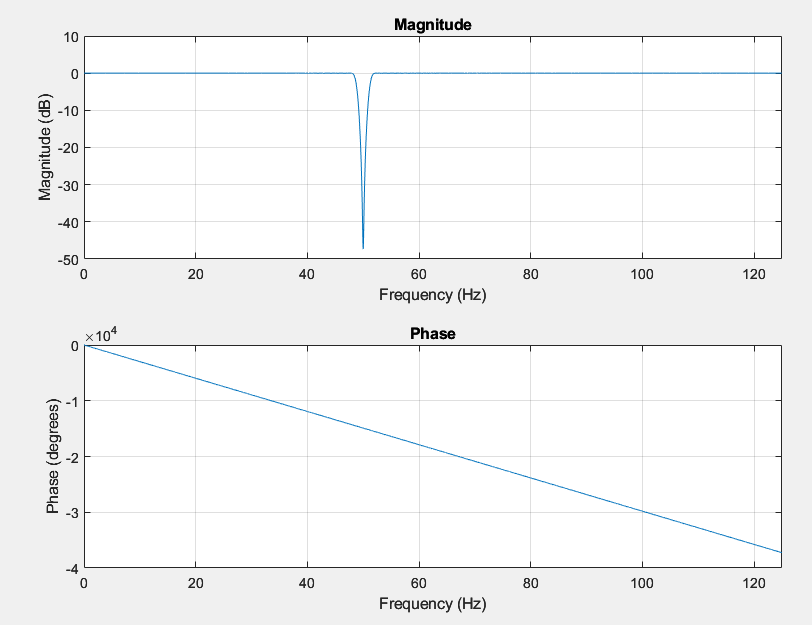
\includegraphics[width=\linewidth]{6}
		\end{subfigure}
		\caption{Notch filter}
	\end{figure}
	
	By comparing with the original signal, we can see that the filtered signal is clearer.
	
	\begin{figure}[!h]
		\centering
		\begin{subfigure}{0.45\textwidth}
			\centering
			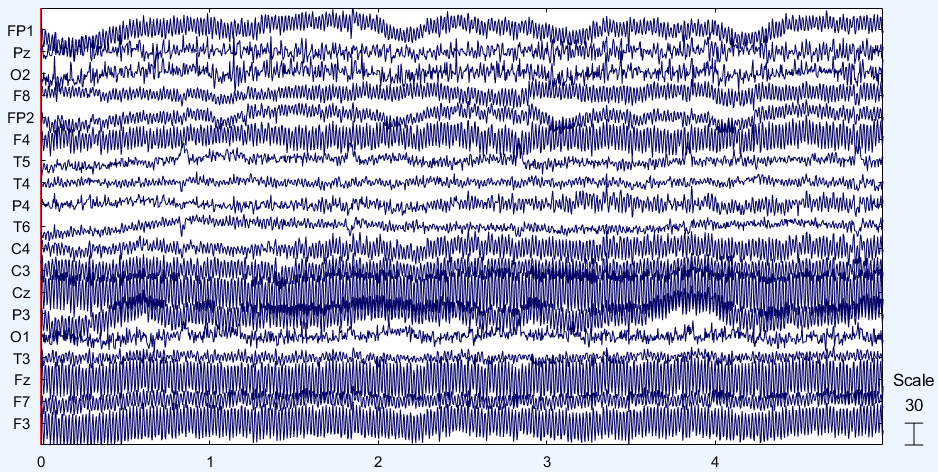
\includegraphics[height=0.52\linewidth]{7}
			\caption{Original signal}
		\end{subfigure}
		\hfill
		\begin{subfigure}{0.45\textwidth}
			\centering
			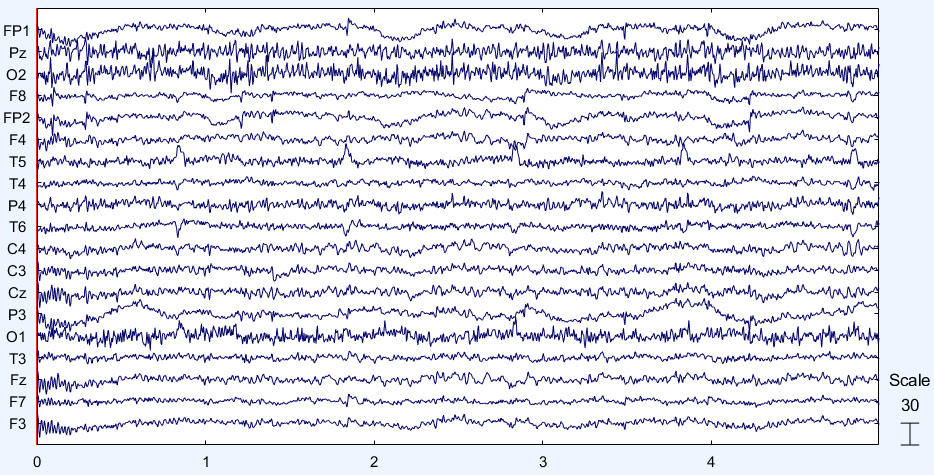
\includegraphics[height=0.52\linewidth]{8}
			\caption{Filtered signal}
		\end{subfigure}
	\end{figure}
	
	\newpage
	
	
	\subsection{Identify and Remove Noisy Channels}
		In this step, we use clean\textunderscore rawdata() to detect and exclude noisy or flatline channels. Since our sensors are spatially adjacent, the brain wave passing through each one has to have a high correlation with its neighbors. Therefore, we set the minimum acceptable correlation to 0.8 (meaning if it is lower, the channel will be removed).

		Tools > Reject data using Clean Rawdata and ASR
		
		\begin{figure}[h!]
			\centering
			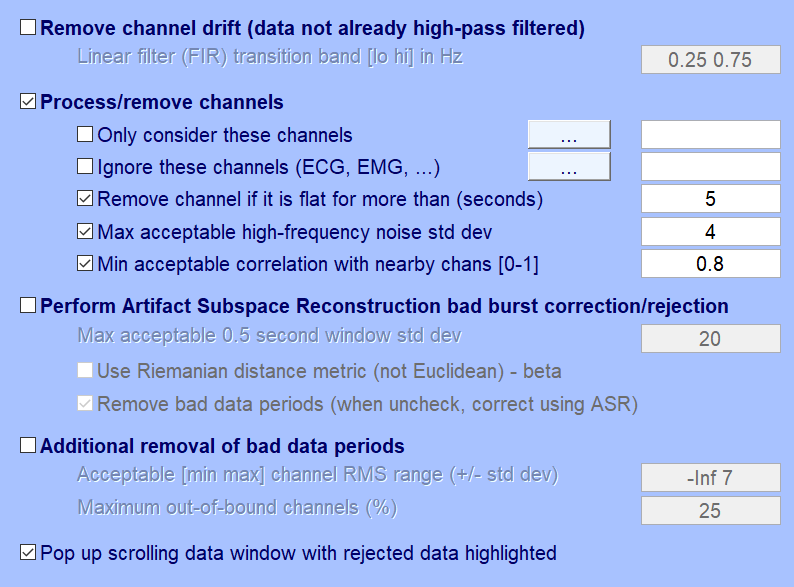
\includegraphics[width=0.4\textwidth]{9}
			\caption{Removing noisy channels}
		\end{figure}
		
	After applying this function, we find out channels "Pz" and "P3" are noisy and have to be removed.
		
		\begin{figure}[h!]
			\centering
			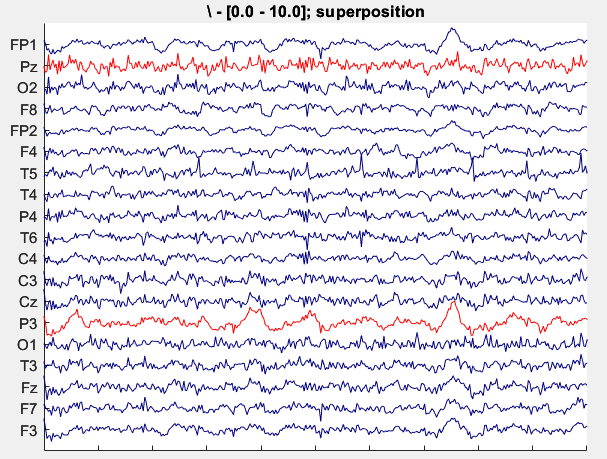
\includegraphics[width=0.4\textwidth]{10}
			\caption{Deleted channels}
		\end{figure}
		
		
		\begin{figure}[!h]
			\centering
			\begin{subfigure}{0.3\textwidth}
				\centering
				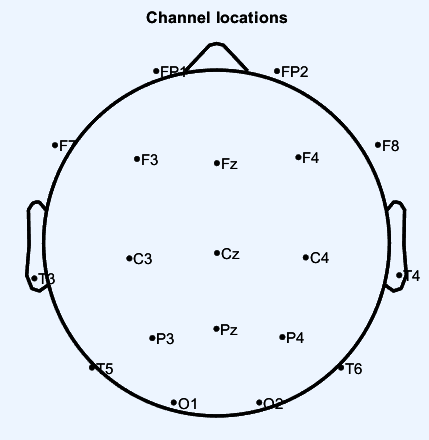
\includegraphics[width=\linewidth]{13}
				\caption{Before removal}
			\end{subfigure}
			\hspace{1cm}
			\begin{subfigure}{0.3\textwidth}
				\centering
				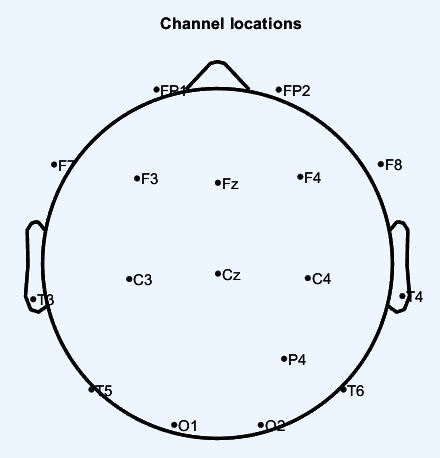
\includegraphics[width=\linewidth]{14}
				\caption{After removal}
			\end{subfigure}
		\end{figure}
		
	\newpage
	
	\subsection{Interpolate Removed Channels}
		Since we need a complete set of channels, we interpolate the removed channels.
		
		Tools > Interpolate electrodes
		
		\begin{figure}[h!]
			\centering
			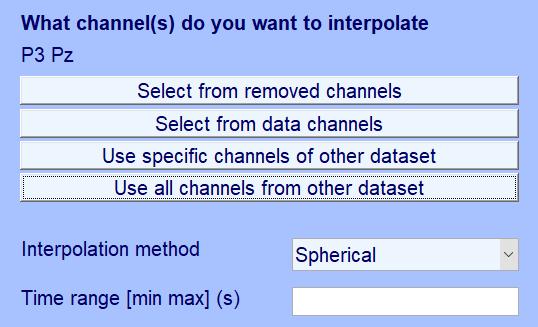
\includegraphics[width=0.35\textwidth]{11}
		\end{figure}
		
		
		
	\subsection{Re-reference EEG (First Pass)}
		We re-reference signals to the average of all EEG channels to remove common-mode noise.
		
		Tools > Re-reference the data
		
		\begin{figure}[h!]
			\centering
			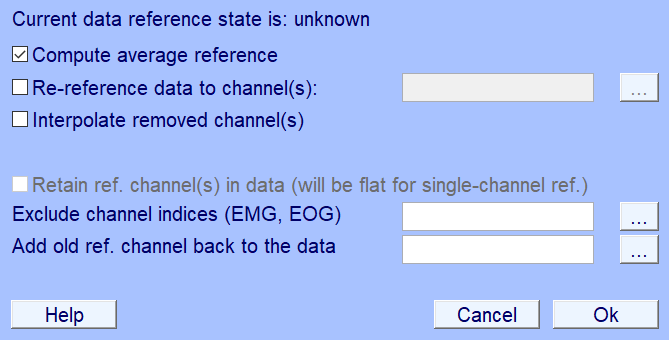
\includegraphics[width=0.35\textwidth]{12}
		\end{figure}
	
	\subsection{Artifact Subspace Reconstruction (ASR)}
		We apply ASR to eliminate transient artifacts such as blinking or frowning.
		
		Tools > Reject data using Clean Rawdata and ASR
		
		\begin{figure}[h!]
			\centering
			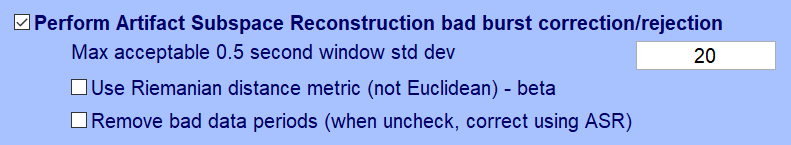
\includegraphics[width=0.5\textwidth]{16}
		\end{figure}
		
		\begin{figure}[h!]
			\centering
			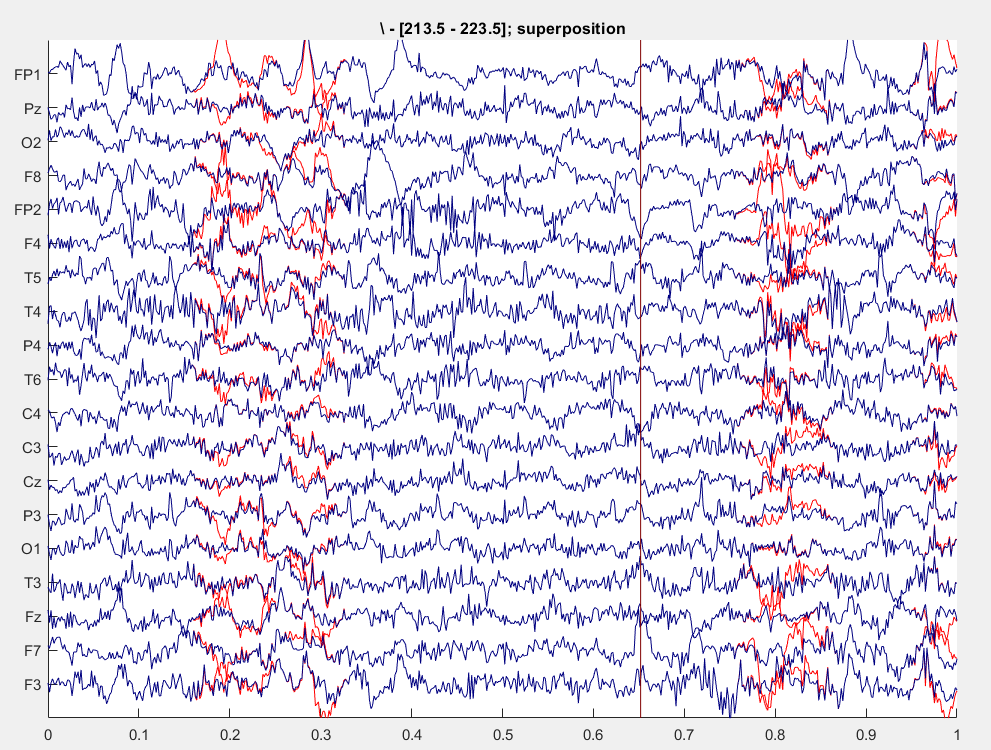
\includegraphics[width=0.5\textwidth]{17}
			\caption{blue: cleaned - red: original}
		\end{figure}
	
	\newpage
	
	\subsection{Re-reference EEG (Second Pass)}
	
		In this step, we perform a second average re-referencing post-ASR for normalization.
		
	
	\subsection{Independent Component Analysis (ICA)}
		First, we check and fit our channels to a standard head model.
		
		Tools > Source localization using DIPFIT > Head model and settings
		
		\begin{figure}[h!]
			\centering
			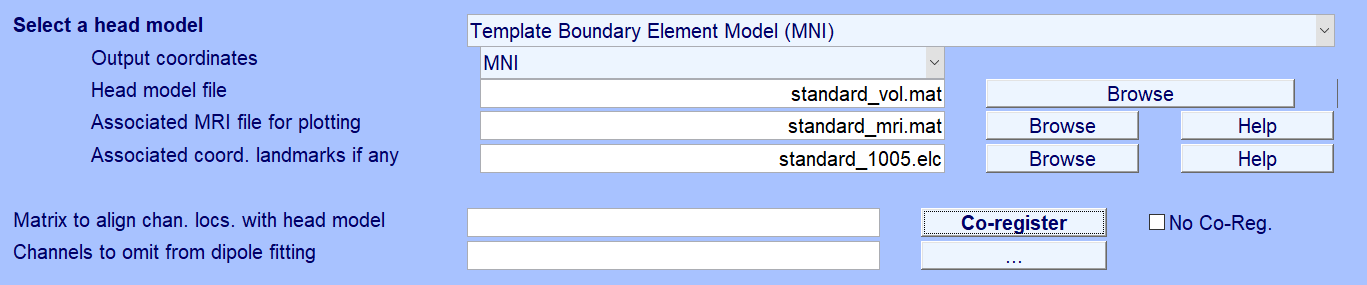
\includegraphics[width=0.7\textwidth]{18}
		\end{figure}
	
		We select MNI and click Co-register. For the channels to be placed properly, we select Wrap Montage.
		
		\begin{figure}[!h]
			\centering
			\begin{subfigure}{0.3\textwidth}
				\centering
				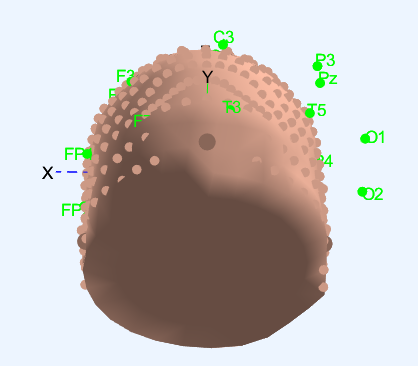
\includegraphics[width=\linewidth]{19}
				\caption{Before wrap montage}
			\end{subfigure}
			\hspace{1cm}
			\begin{subfigure}{0.3\textwidth}
				\centering
				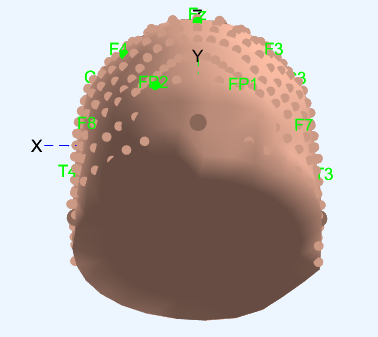
\includegraphics[width=\linewidth]{20}
				\caption{After wrap montage}
			\end{subfigure}
		\end{figure}
		
		Now we are ready to decompose our data using ICA. ICA assumes that our signal sources are independent, as we have enough samples, and assigns a weight to the effect of each source on our signal.
		
		Tools > Decompose data by ICA
		
		\begin{figure}[h!]
			\centering
			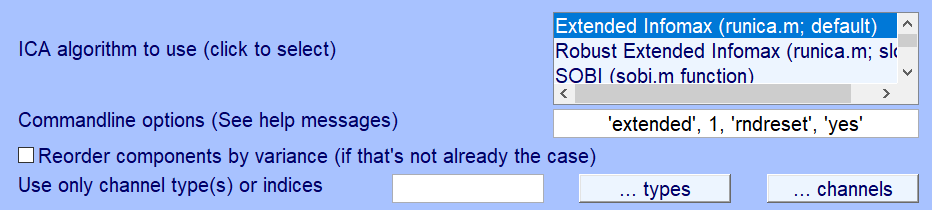
\includegraphics[width=0.7\textwidth]{21}
		\end{figure}
		
		We should choose the ICA rank carefully, since we removed a number of channels. Then, we fit dipoles to our ICs.
		
		\begin{figure}[h!]
			\centering
			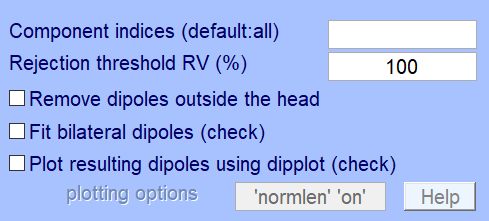
\includegraphics[width=0.4\textwidth]{22}
		\end{figure}
				
		\newpage
		
		After fitting single dipoles, we attempt to fit bilateral dipoles.
		
		\begin{figure}[h!]
			\centering
			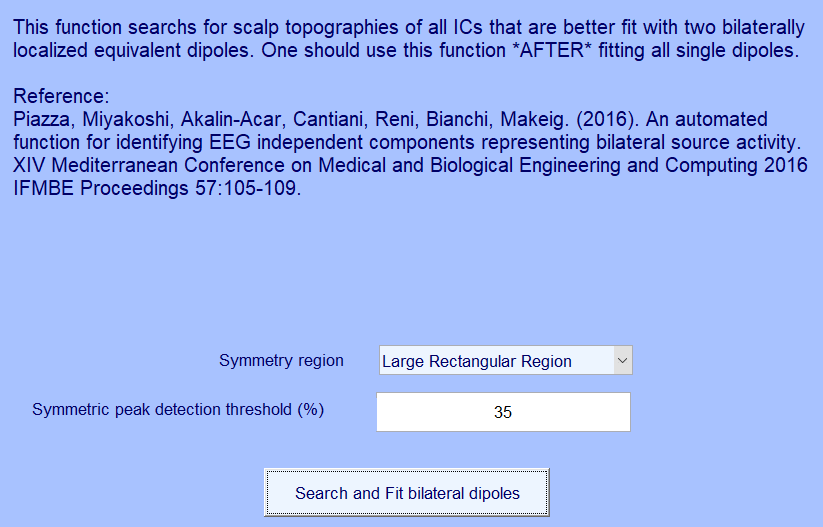
\includegraphics[width=0.4\textwidth]{23}
		\end{figure}
		
		Finally, we can view our components.
		
		\begin{figure}[h!]
			\centering
			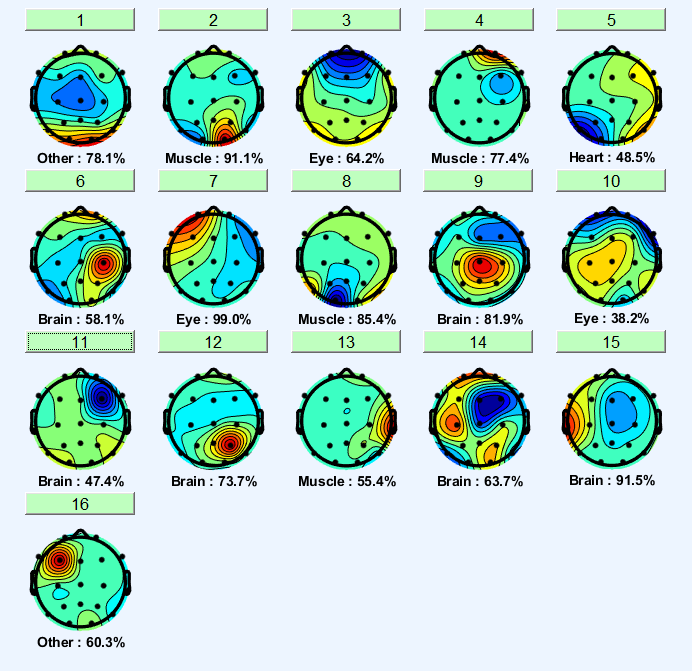
\includegraphics[width=0.6\textwidth]{24}
		\end{figure}
		
		We inspect each component and then remove those identified as artifacts. Muscle ICs are typically superficial and concentrated on one electrode. The following ICs are suspected to be muscle-related.
		
		\begin{figure}[!h]
			\centering
			\begin{subfigure}{0.45\textwidth}
				\centering
				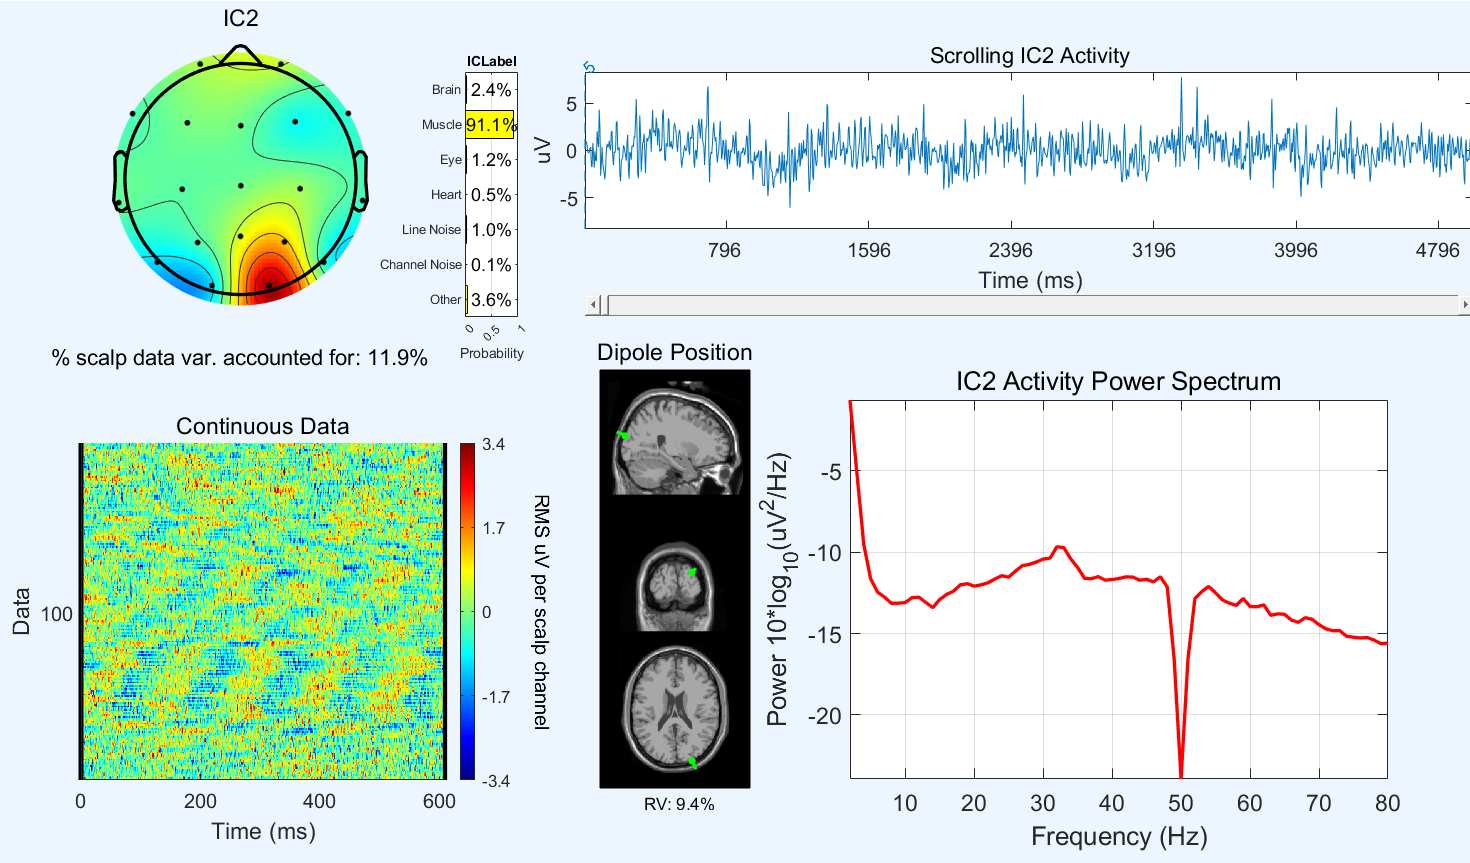
\includegraphics[width=\linewidth]{hc/2}
			\end{subfigure}
			\hfill
			\begin{subfigure}{0.45\textwidth}
				\centering
				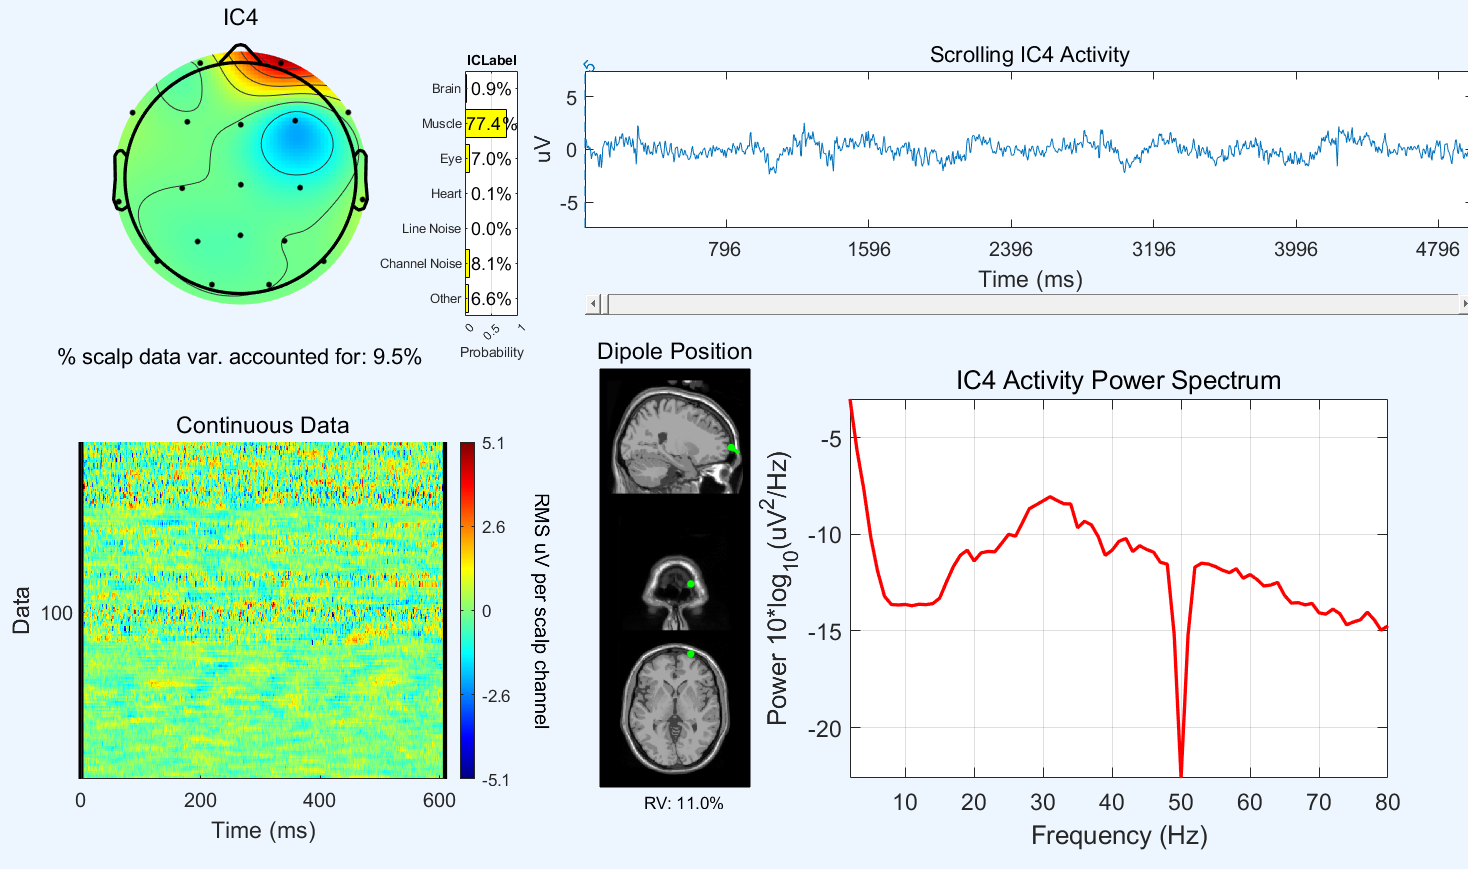
\includegraphics[width=\linewidth]{hc/4}
			\end{subfigure}
		\end{figure}
		
		\newpage

		\begin{figure}[!h]
			\centering
			\begin{subfigure}{0.45\textwidth}
				\centering
				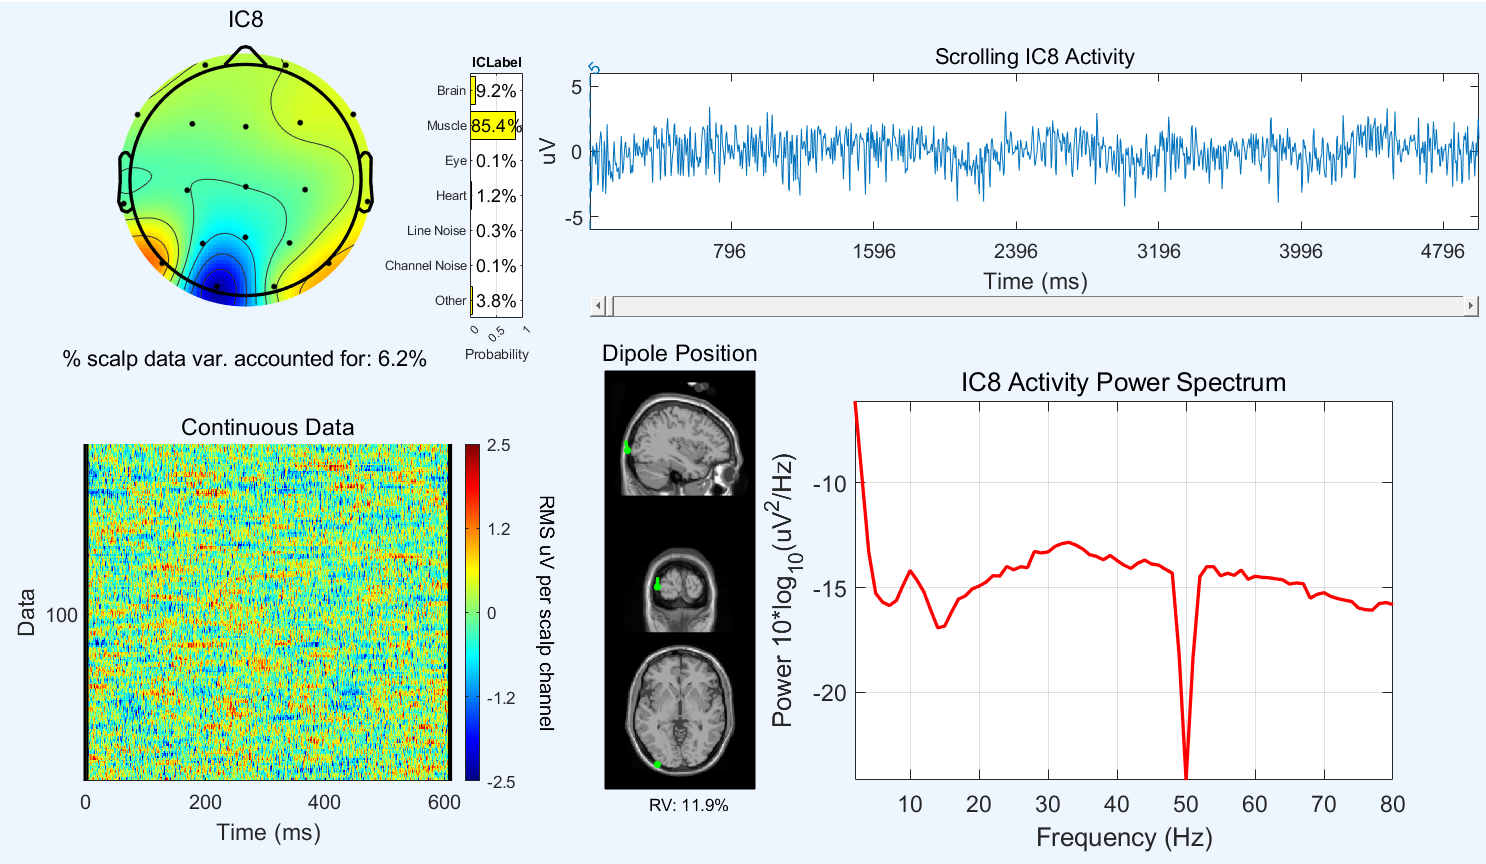
\includegraphics[width=\linewidth]{hc/8}
			\end{subfigure}
			\hfill
			\begin{subfigure}{0.45\textwidth}
				\centering
				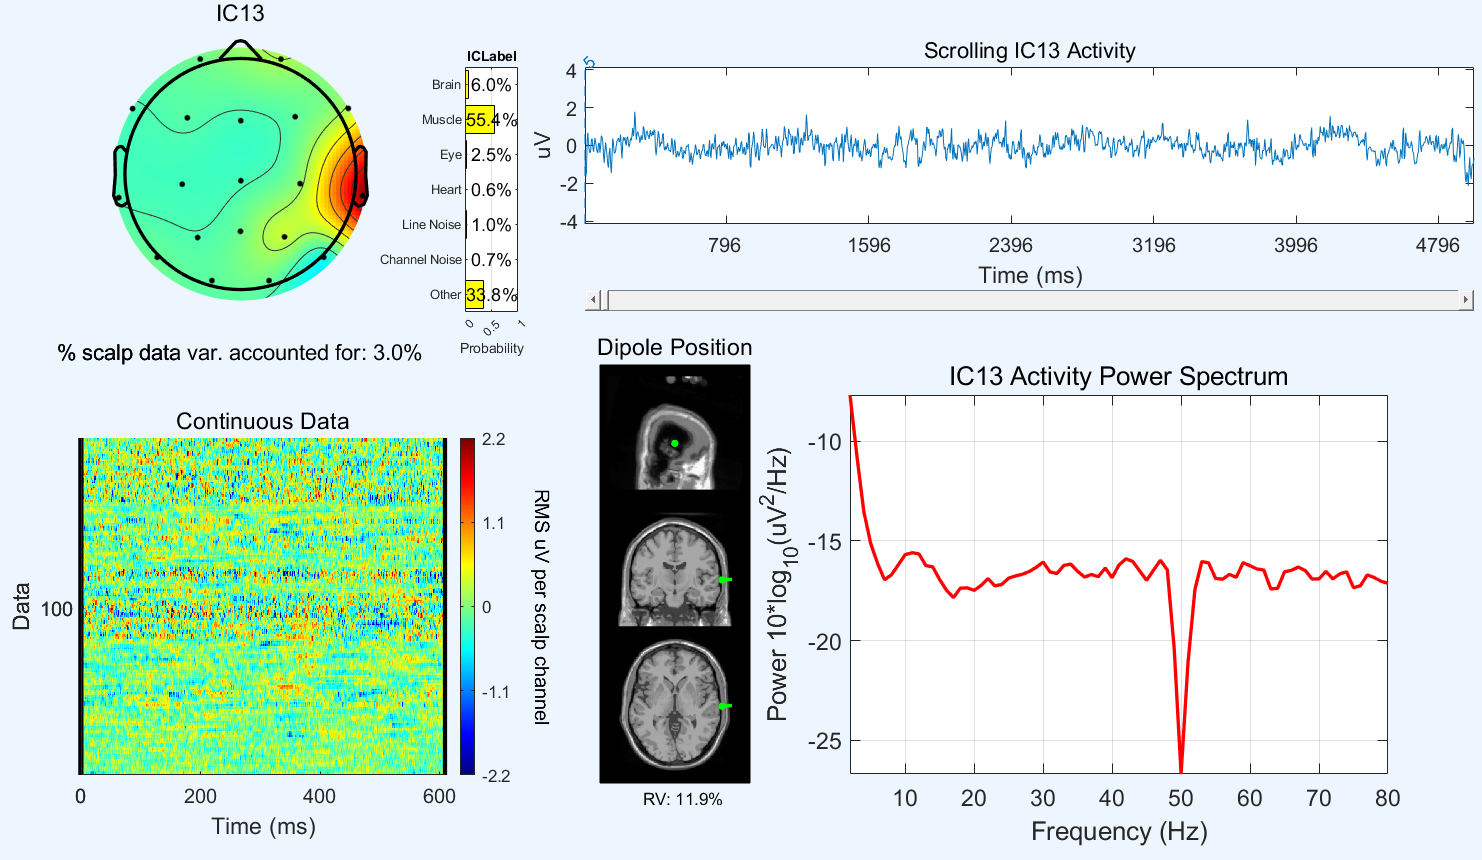
\includegraphics[width=\linewidth]{hc/13}
			\end{subfigure}
		\end{figure}
	
	After removing the artifact components, we obtain the following signal.
	
	\begin{figure}[h!]
		\centering
		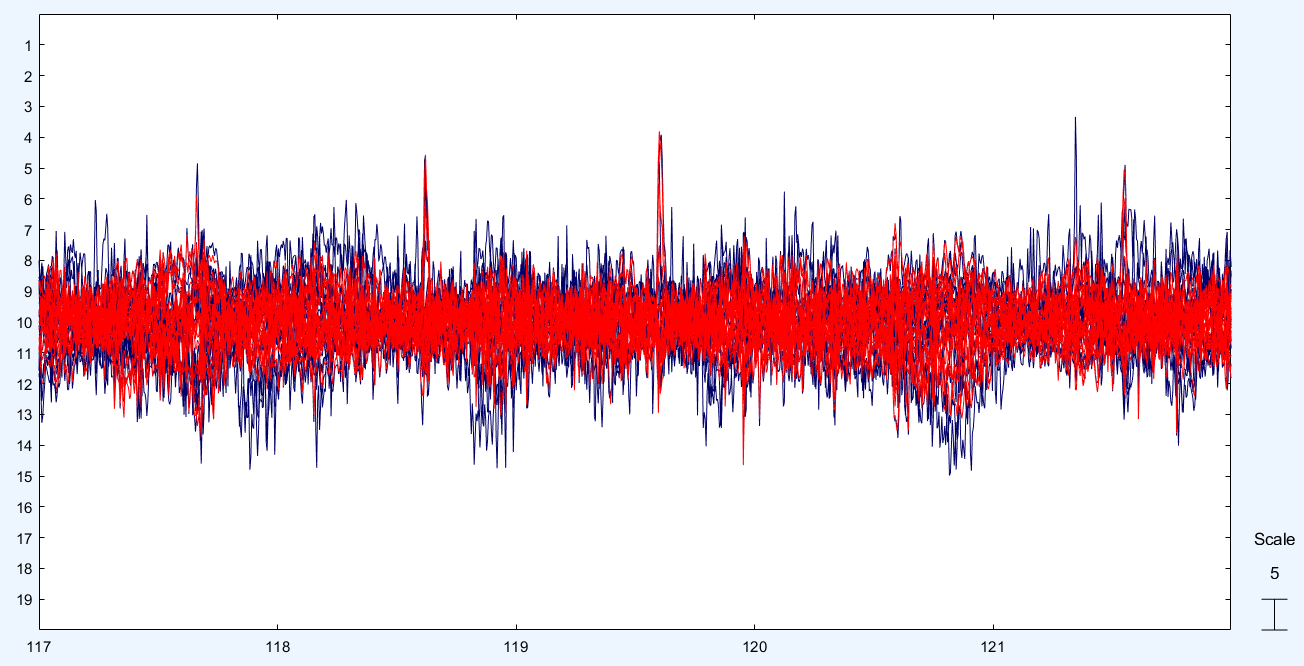
\includegraphics[width=0.7\textwidth]{25}
		\caption{black: before rejection - red: after rejection}
	\end{figure}
	
	We can see that our final signal is much cleaner than the original.
	
	\begin{figure}[!h]
		\centering
		\begin{subfigure}{0.45\textwidth}
			\centering
			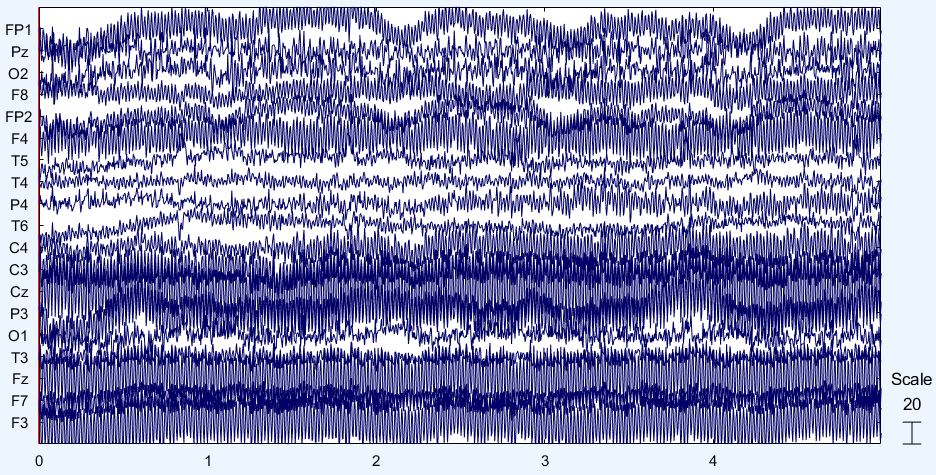
\includegraphics[width=\linewidth]{26}
			\caption{original}
		\end{subfigure}
		\hfill
		\begin{subfigure}{0.45\textwidth}
			\centering
			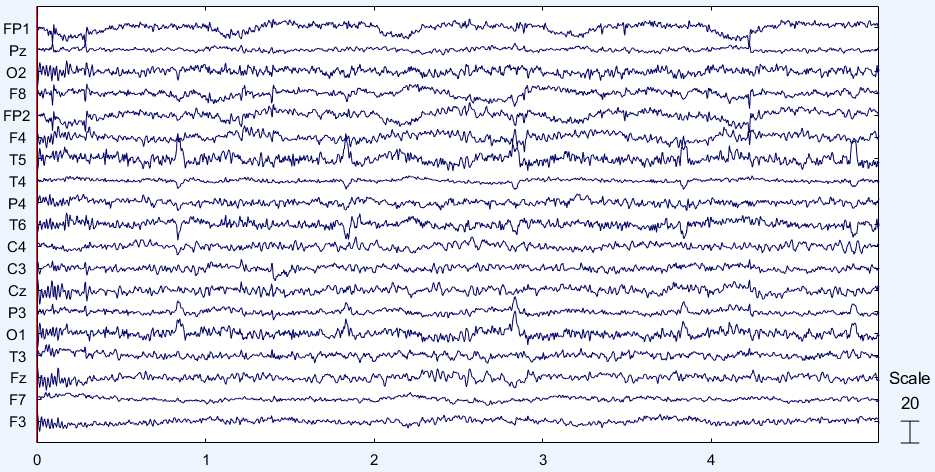
\includegraphics[width=\linewidth]{27}
			\caption{pre-processed}
		\end{subfigure}
	\end{figure}
	
	\subsection{Epoching}
		We segment trials from -2 to +5 seconds around odor onset to capture pre-stimulus, stimulus, and post-stimulus dynamics.
		
		\begin{figure}[h!]
			\centering
			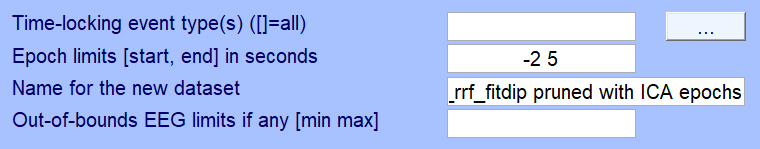
\includegraphics[width=0.6\textwidth]{28}
		\end{figure}


	\subsection{Trial Rejection}
		For the final step, we use Automatic Epoch Rejection to rule out noisy trials.
		\begin{figure}[h!]
			\centering
			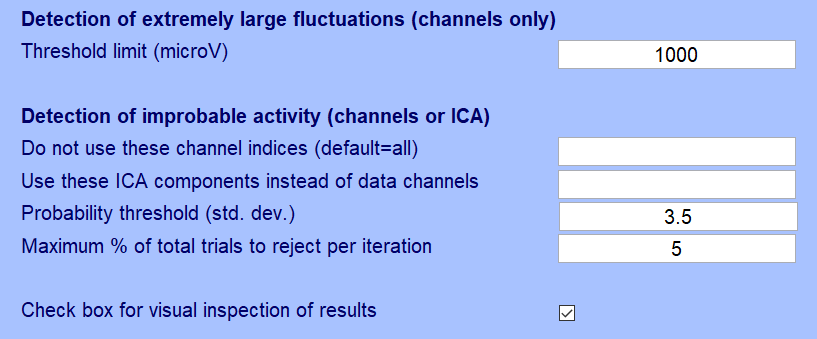
\includegraphics[width=0.5\textwidth]{29}
		\end{figure}
		
		In this dataset, there were no abnormal trials to remove.
	\newpage
	
	\section{Mild Cognitive Impairment}
	
	Since most of the preprocessing pipeline is similar to the previous one, we will only mention the steps that differ.
	
	\subsection{Identify and Remove Noisy Channels}
	Here, we cannot set the correlation to 0.8 since both FP1 and FP2 are spatially adjacent, and their removal would result in information loss that cannot be interpolated. Therefore, we set the correlation threshold to 0.7.

	\begin{figure}[!h]
		\centering
		\begin{subfigure}{0.45\textwidth}
			\centering
			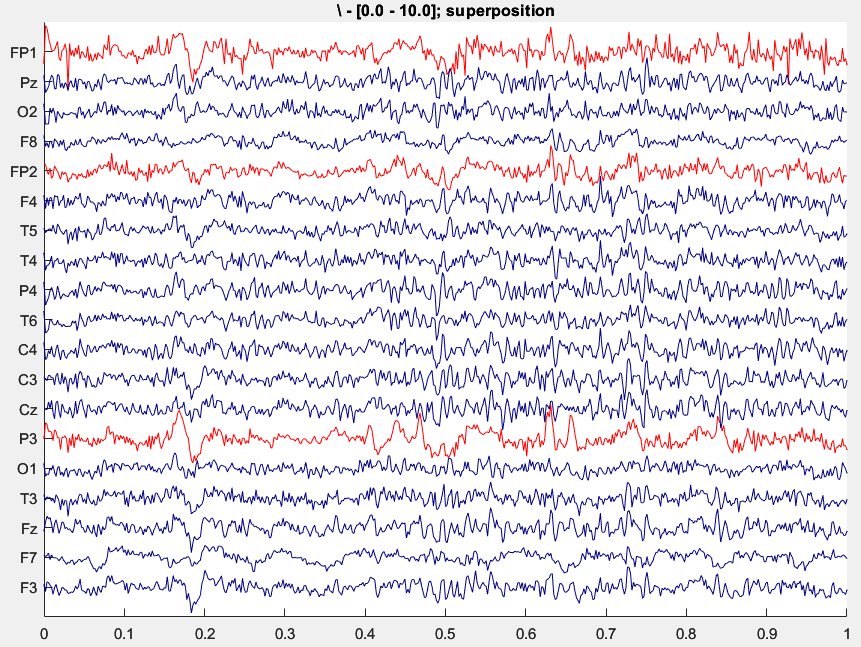
\includegraphics[height=0.8\linewidth]{30}
			\caption{std = 3.5 - $\rho$ = 0.8}
		\end{subfigure}
		\hspace{1cm}
		\begin{subfigure}{0.45\textwidth}
			\centering
			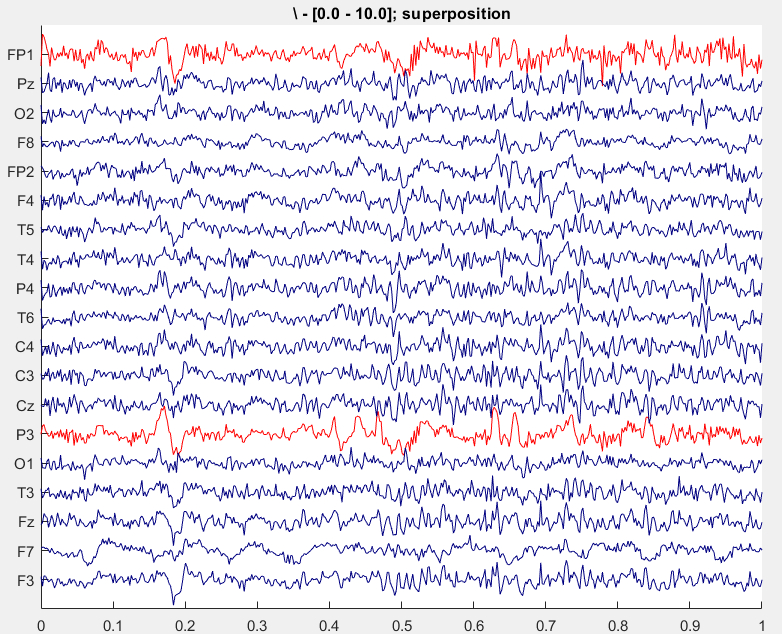
\includegraphics[height=0.8\linewidth]{31}
			\caption{std = 3.5 - $\rho$ = 0.7}
		\end{subfigure}
	\end{figure}
	
	\begin{figure}[h!]
		\centering
		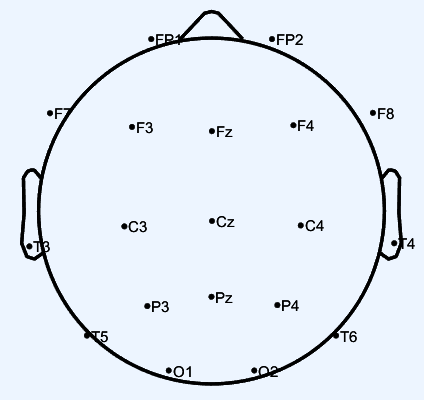
\includegraphics[width=0.4\textwidth]{32}
		\caption{Channel locations}
	\end{figure}
	
	\newpage
	
	\subsection{Independent Component Analysis (ICA)}
	\begin{figure}[h!]
		\centering
		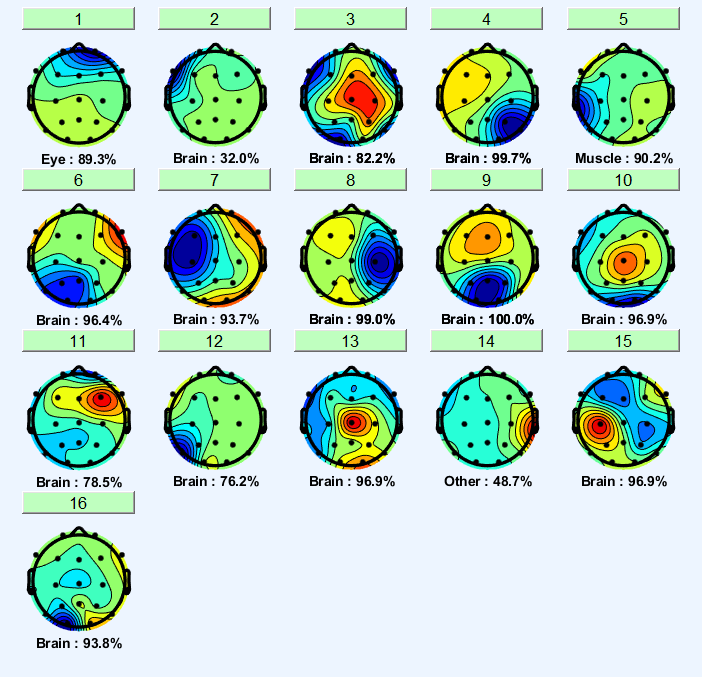
\includegraphics[width=0.7\textwidth]{33}
		\caption{Components}
	\end{figure}
	
	\begin{figure}[h!]
		\centering
		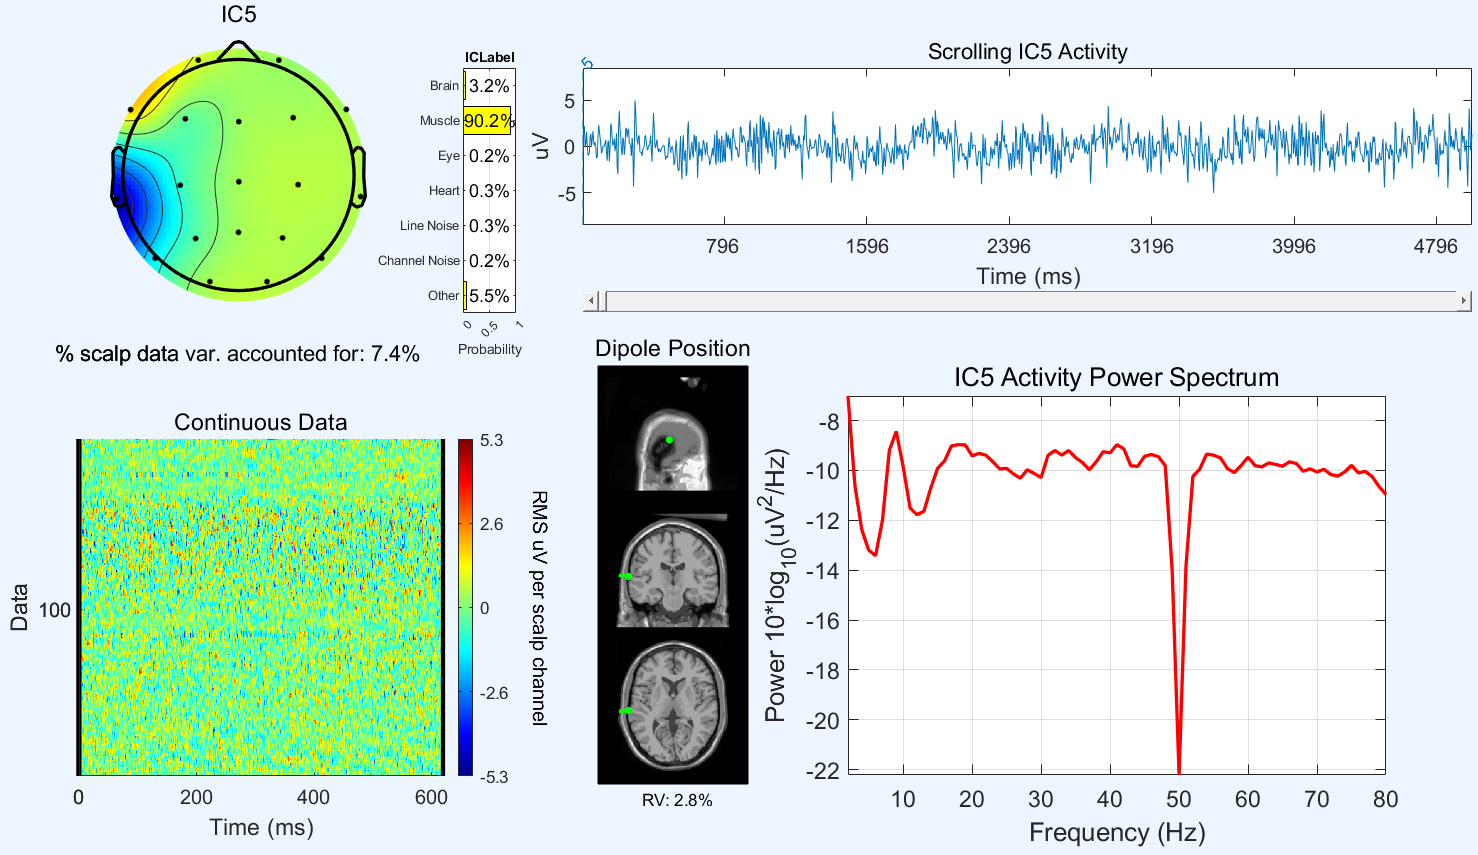
\includegraphics[width=0.9\textwidth]{mci/5}
		\caption{Removed component}
	\end{figure}
	
	
	\newpage
	
	\subsection{Trial Rejection}
	
	\begin{figure}[h!]
		\centering
		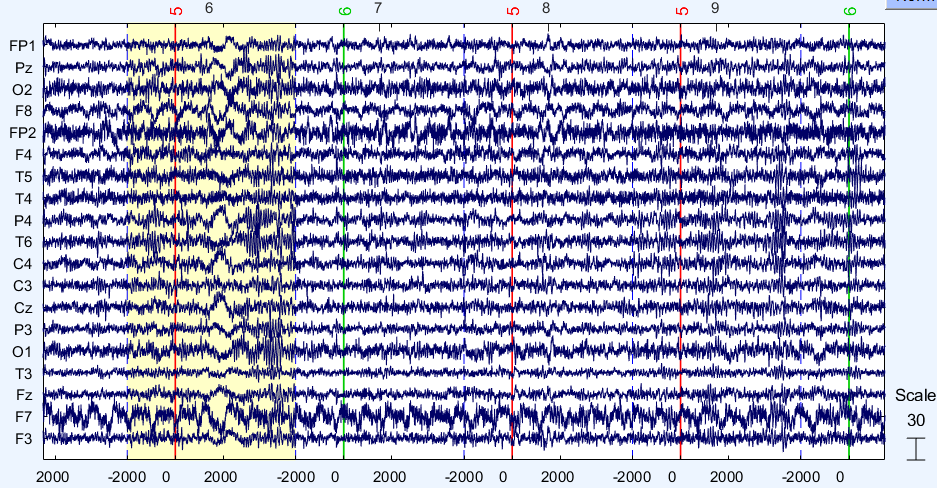
\includegraphics[width=0.7\textwidth]{34}
	\end{figure}
	
	\begin{figure}[h!]
		\centering
		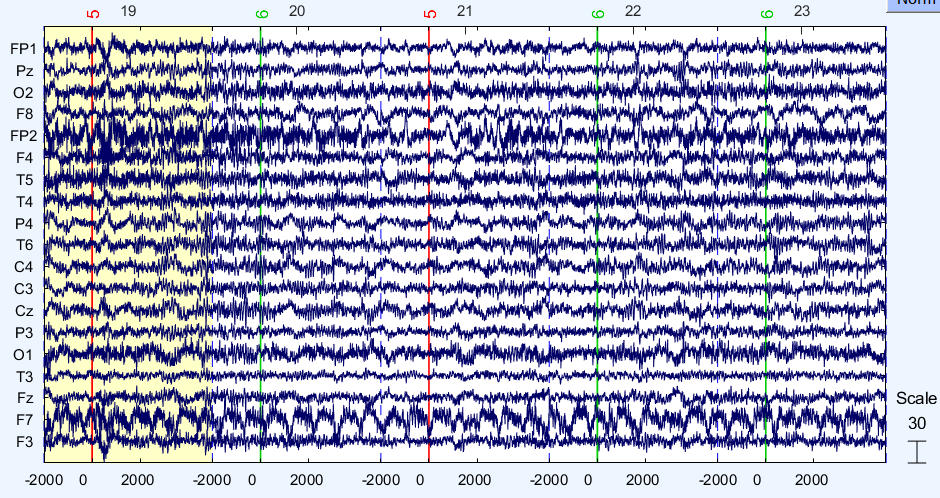
\includegraphics[width=0.7\textwidth]{35}
	\end{figure}
	
	\begin{figure}[h!]
		\centering
		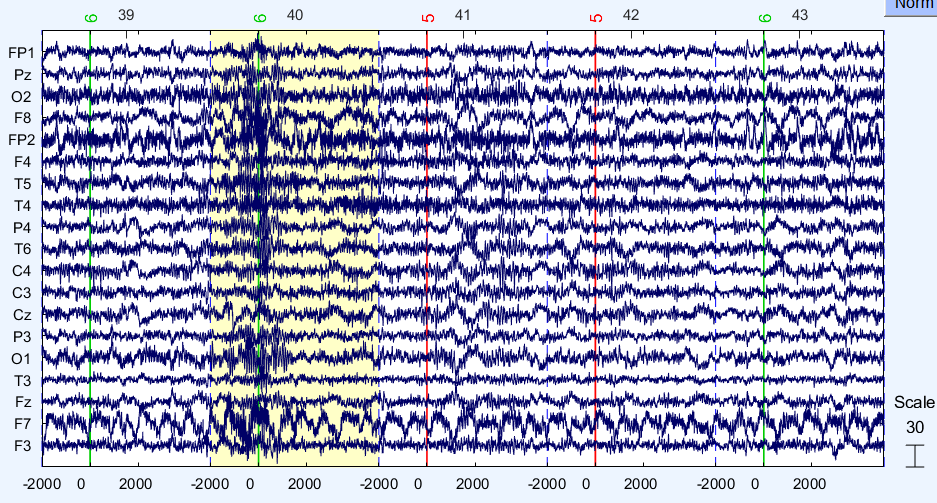
\includegraphics[width=0.7\textwidth]{36}
		\caption{Removed trials}
	\end{figure}
	
	\newpage
	
	
	\section{Mild Alzheimer's Disease}
	\subsection{Identify and Remove Noisy Channels}
	The situation is the same as before. We cannot set the correlation threshold to 0.8 because six of our channels would be lost.
	\begin{figure}[!h]
		\centering
		\begin{subfigure}{0.45\textwidth}
			\centering
			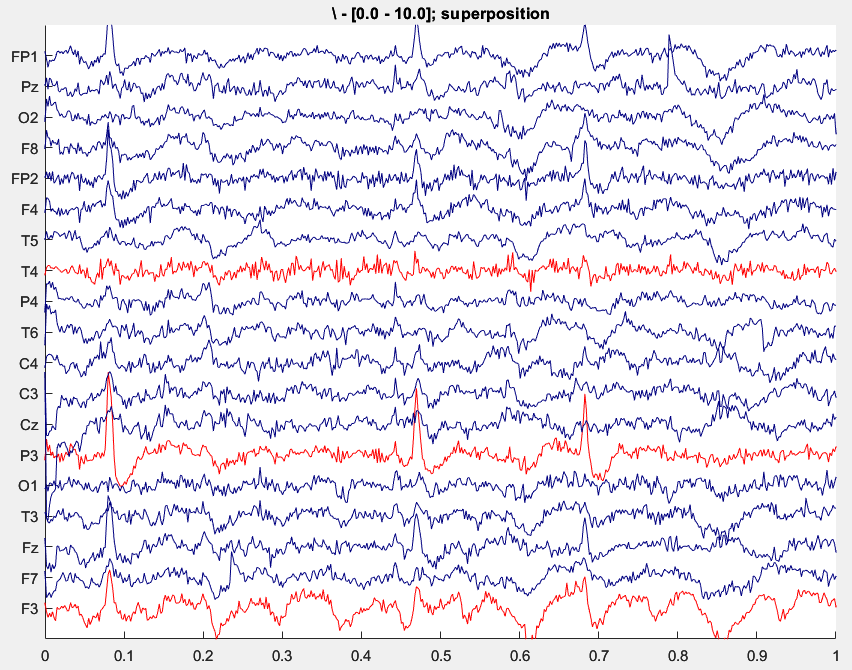
\includegraphics[height=0.8\linewidth]{37}
			\caption{std = 4 - $\rho$ = 0.75}
		\end{subfigure}
		\hspace{1cm}
		\begin{subfigure}{0.45\textwidth}
			\centering
			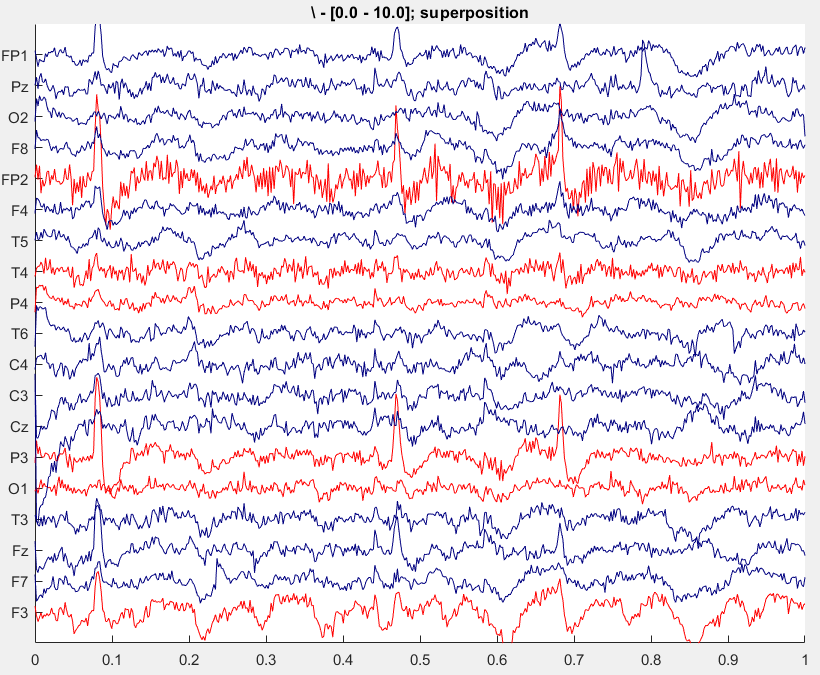
\includegraphics[height=0.8\linewidth]{38}
			\caption{std = 4 - $\rho$ = 0.8}
		\end{subfigure}
	\end{figure}
	
	\subsection{Independent Component Analysis (ICA)}
	\begin{figure}[h!]
		\centering
		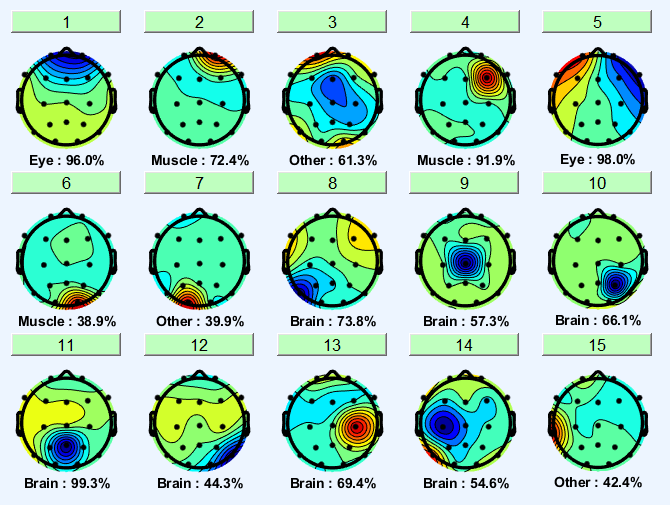
\includegraphics[width=0.7\textwidth]{39}
		\caption{Components}
	\end{figure}
	
	\begin{figure}[!h]
		\centering
		\begin{subfigure}{0.4\textwidth}
			\centering
			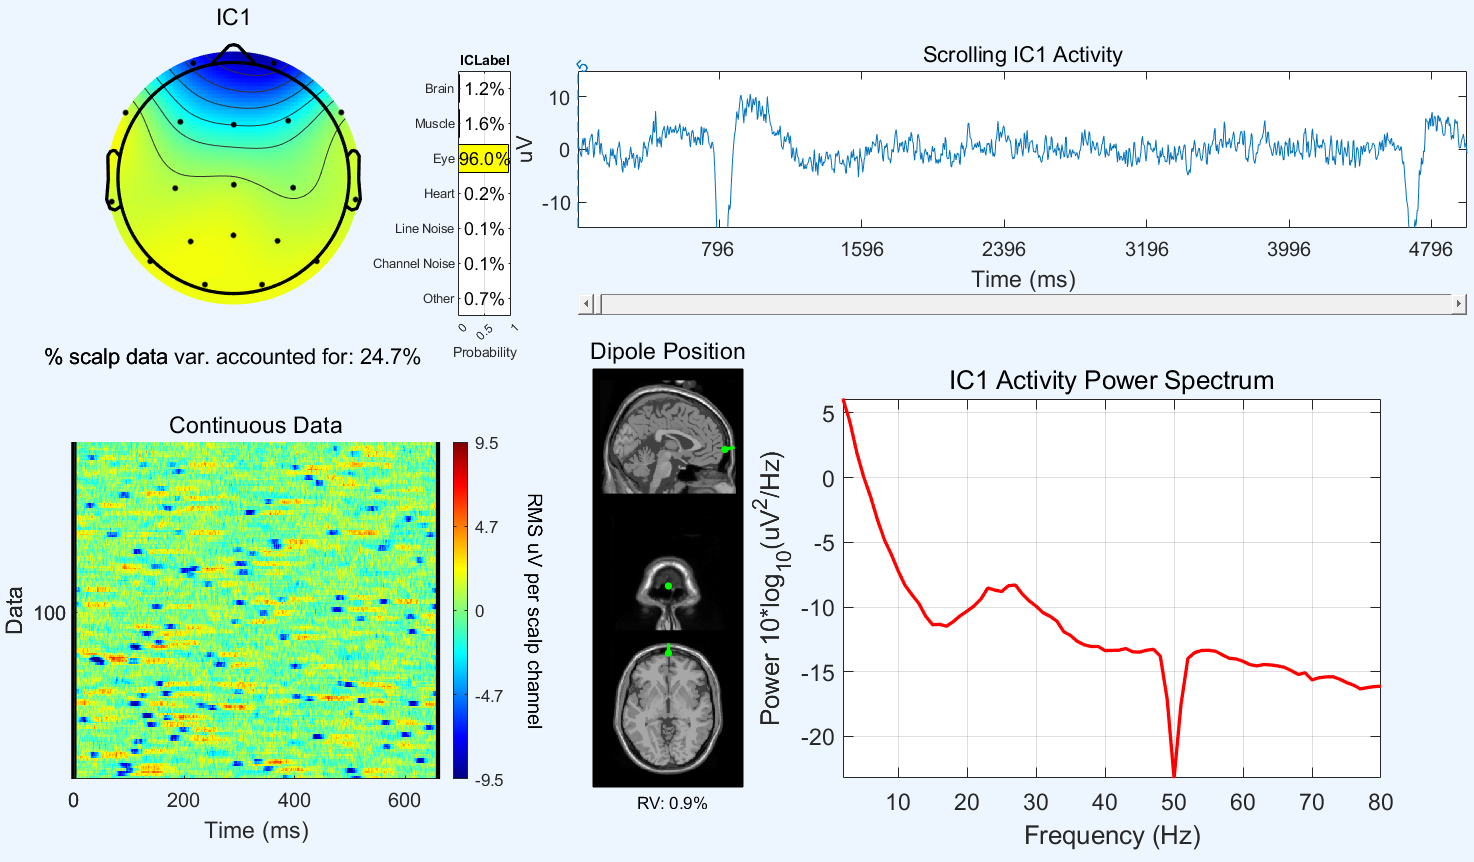
\includegraphics[width=\linewidth]{mc/1}
		\end{subfigure}
		\hspace{1cm}
		\begin{subfigure}{0.4\textwidth}
			\centering
			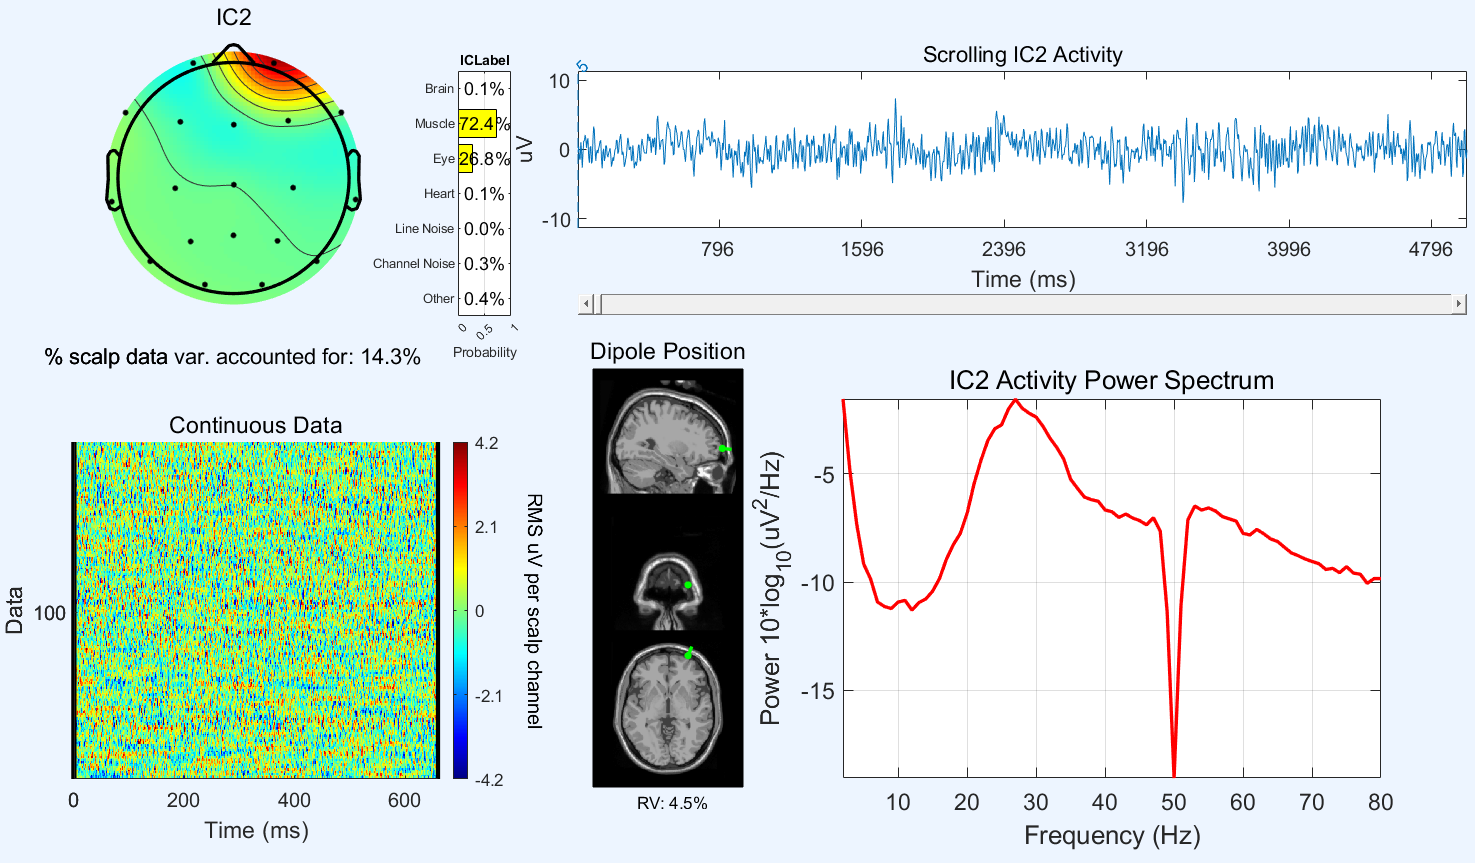
\includegraphics[width=\linewidth]{mc/2}
		\end{subfigure}
	\end{figure}
	
	\newpage
	
	\begin{figure}[!h]
		\centering
		\begin{subfigure}{0.4\textwidth}
			\centering
			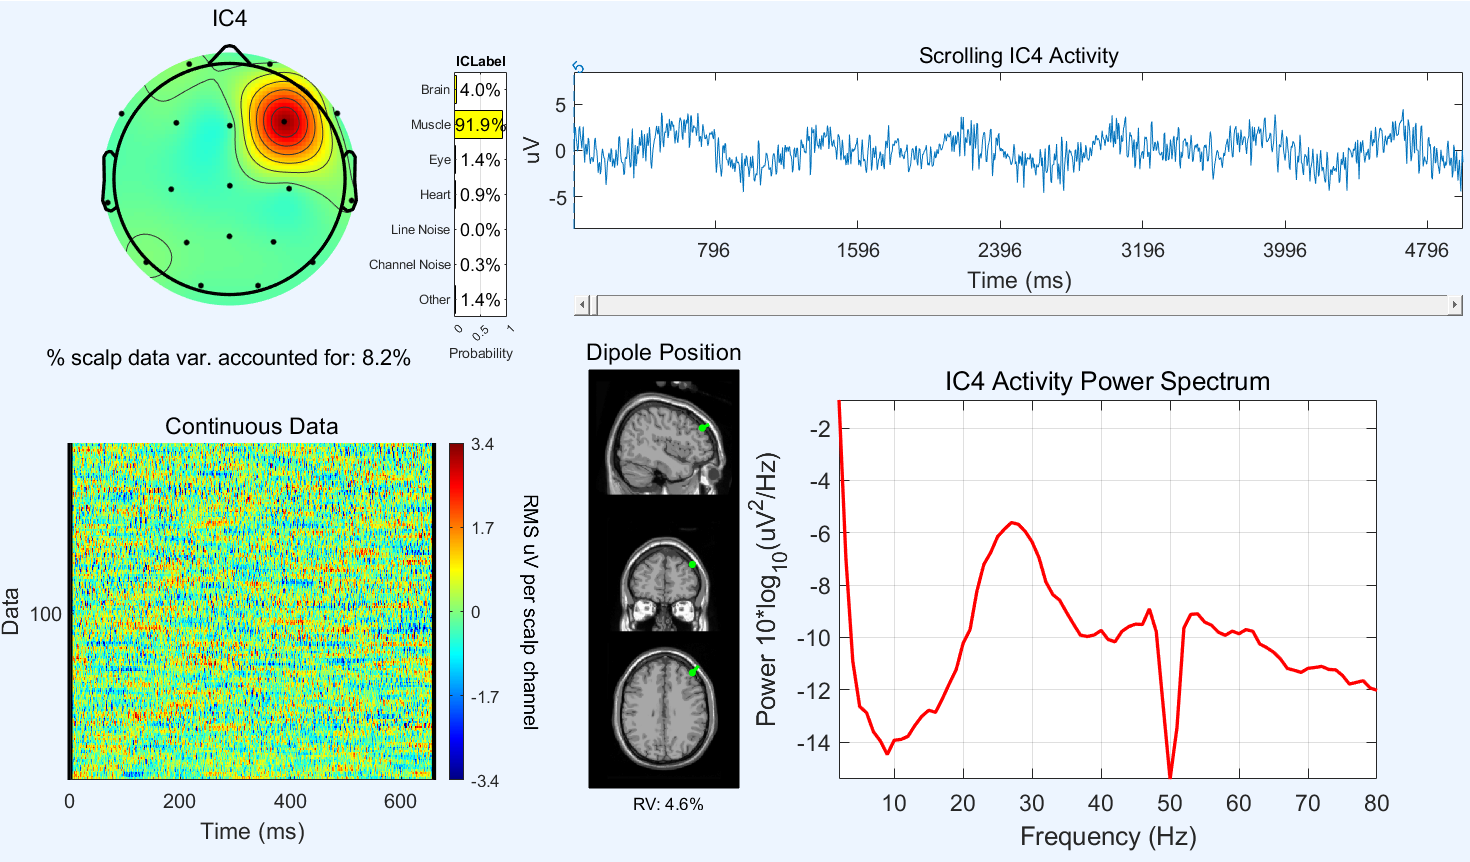
\includegraphics[width=\linewidth]{mc/4}
		\end{subfigure}
		\hspace{1cm}
		\begin{subfigure}{0.4\textwidth}
			\centering
			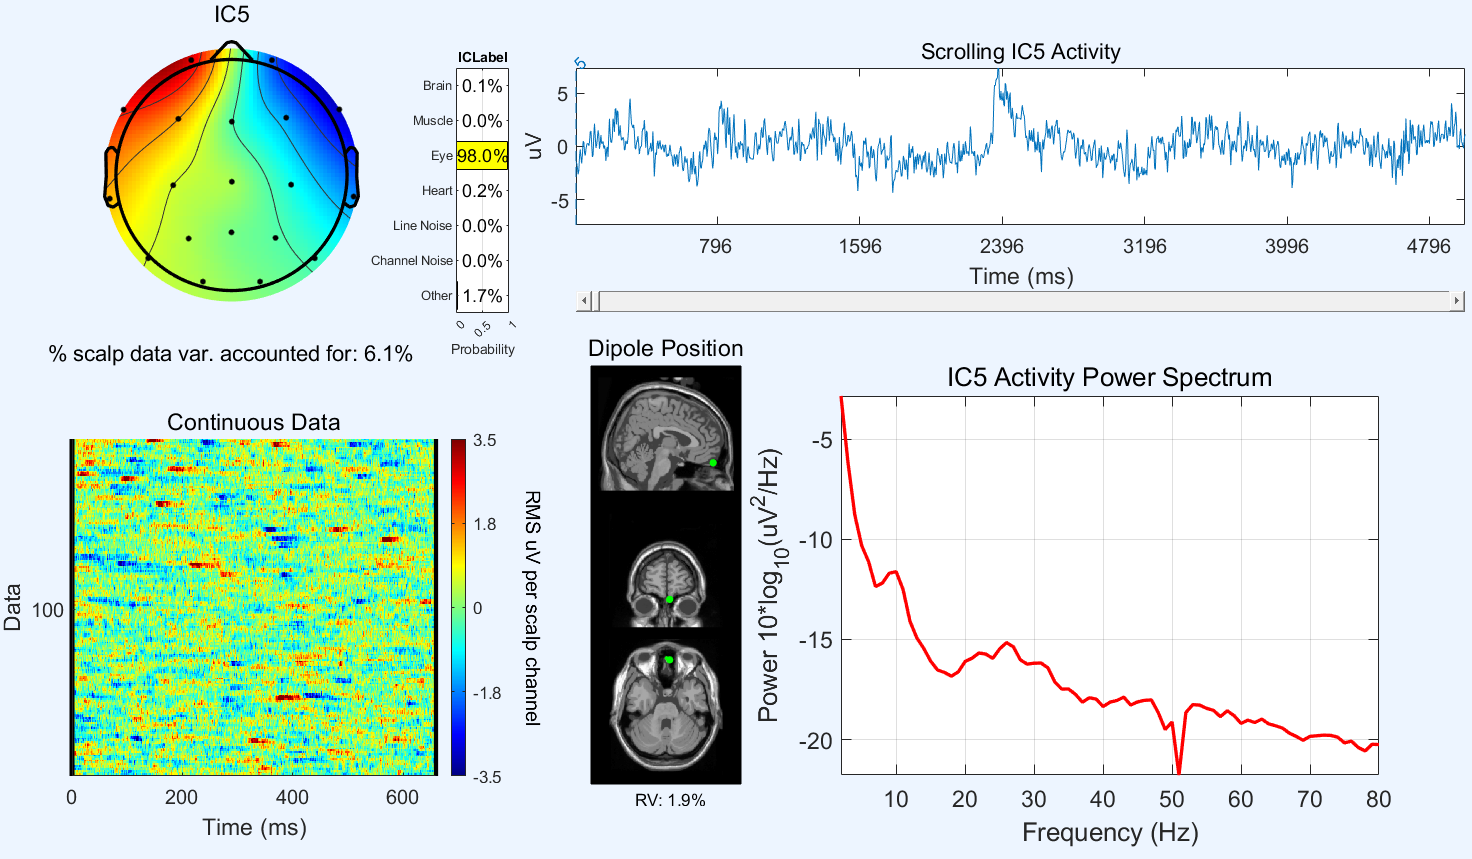
\includegraphics[width=\linewidth]{mc/5}
		\end{subfigure}
		\caption{Removed Components}
	\end{figure}
	
	\begin{figure}[h!]
		\centering
		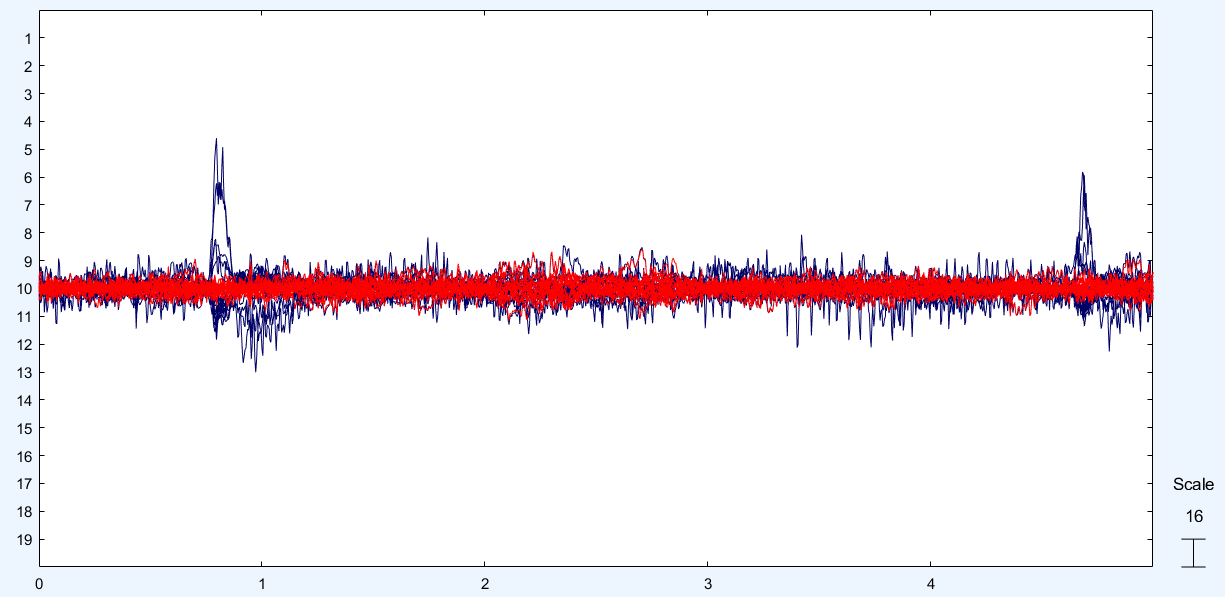
\includegraphics[width=0.6\textwidth]{40}
		\caption{black: before rejection - red: after rejection}
	\end{figure}
	
	\subsection{Trial Rejection}
	\begin{figure}[h!]
		\centering
		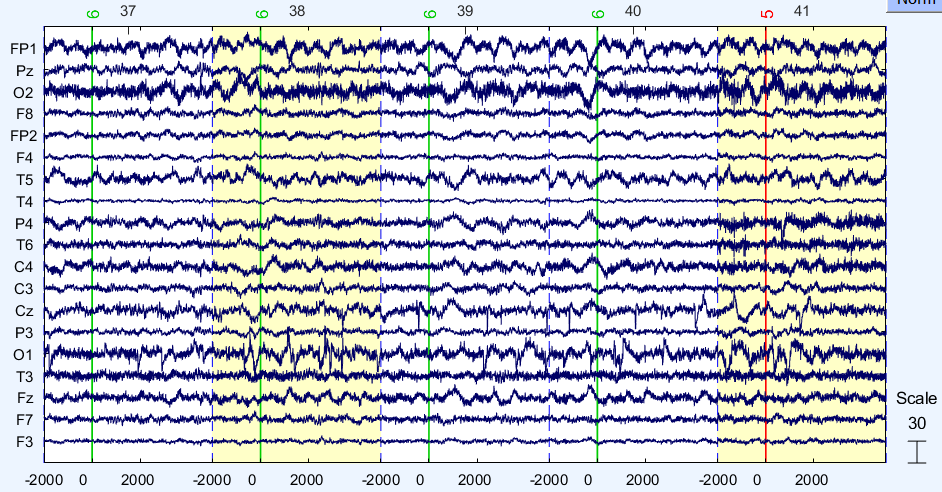
\includegraphics[width=0.6\textwidth]{41}
		\caption{Removed trials}
	\end{figure}
	
	\newpage
	
	\section{Choosing Window Length and Overlap}
	Here we try to see the effect of window length and overlap.
	\begin{figure}[h!]
		\centering
		\includegraphics[width=0.95\textwidth]{42}
		\caption{}
	\end{figure}
	
	We observe that as we move from the top to the bottom, the timing resolution gets lower and more smeared. This shows that the shorter the window length, the clearer the timing resolution. If we look at it from the frequency perspective, it is the exact opposite. We see more distinct lines at the bottom than at the top. This shows that as we increase the window length, we increase the frequency resolution.
	
	\newpage

	\section{Building Power-Time Matrices and Comparison}
	We average the trials and plot them over time.
	
	\begin{figure}[!h]
		\centering
		\begin{subfigure}{0.48\textwidth}
			\centering
			\includegraphics[height=0.8\linewidth]{plots/1}
		\end{subfigure}
		\hfill
		\begin{subfigure}{0.48\textwidth}
			\centering
			\includegraphics[height=0.8\linewidth]{plots/3}
		\end{subfigure}
		\caption{Theta power}
	\end{figure}
	
	\begin{figure}[!h]
		\centering
		\begin{subfigure}{0.48\textwidth}
			\centering
			\includegraphics[height=0.8\linewidth]{plots/2}
		\end{subfigure}
		\hfill
		\begin{subfigure}{0.48\textwidth}
			\centering
			\includegraphics[height=0.8\linewidth]{plots/4}
		\end{subfigure}
		\caption{Gamma power}
	\end{figure}
	
	\begin{figure}[!h]
		\centering
		\begin{subfigure}{0.32\textwidth}
			\centering
			\includegraphics[height=\linewidth]{plots/5}
			\caption{Healthy Patient}
		\end{subfigure}
		\hfill
		\begin{subfigure}{0.32\textwidth}
			\centering
			\includegraphics[height=\linewidth]{plots/6}
			\caption{MCI Patient}
		\end{subfigure}
		\hfill
		\begin{subfigure}{0.32\textwidth}
			\centering
			\includegraphics[height=\linewidth]{plots/7}
			\caption{AD Patient}
		\end{subfigure}
	\end{figure}
	
	
	
	\section{Interpretation}
	\begin{itemize}
		\item Do any subjects show stronger or earlier peaks in power?
		
		AD subject consistently shows stronger peaks in Gamma Power under both chocolate and rose odor conditions.
		
		\item Are power patterns different for chocolate vs. rose?
		
		Theta Power: The overall power levels and the timing/amplitude of peaks differ between chocolate and rose odors for all three groups. For example, MCI shows stronger peaks in theta power under rose odor than under chocolate odor, while the healthy subject shows a more dramatic shift in peak timing and amplitude.
		
		Gamma Power: The general trend of AD > MCI > Healthy holds for both odors.
		
		\item Is there a consistent delay or drop in response in the MCI or Alzheimer's subjects?
		
		The AD subject demonstrates a consistent drop in theta power, while the healthy subject demonstrates a consistent drop in gamma power. But there are no signs of a delay in AD or MCI responses.
		
		\item Does theta or gamma seem more affected in impaired states?
		
		Gamma power seems to be notably elevated in the Alzheimer's Disease subject and appears more affected.
	\end{itemize}
	
	\subsection{Reflective Questions}
	
	\begin{itemize}
		\item Which method of power extraction gave you clearer or more informative results?
		
		The change in Gamma power seems more noticeable. Thus, it is clearer and more obvious.
		
		\item Did you observe consistent differences in power between subjects or odors?
		
		There is a consistent pattern where the AD subject shows higher gamma power than MCI and Healthy subjects under both chocolate and rose odor conditions. Although the AD subject also consistently shows significantly lower theta power, this difference is less obvious.
		
		\item What preprocessing choices might have influenced your results, and what would you try differently next time?
		
		The initial epoching window was set from -2 to 5 seconds, which captured a good range around the stimulus, but next time I'd like to experiment with different lengths. For bandpass filtering, we had to use a 1 to 90 Hz range. I'm curious to see how a narrower 1 to 70 Hz range affects our results. Finally, I'd want to try a stricter standard deviation setting on ASR to achieve an even cleaner signal if possible.
		
		\newpage
		
		
		\item How do these power dynamics set the stage for phase-amplitude coupling in the next phase?
		
		The clear power dynamics we've observed in theta and gamma, particularly how they diverge in AD, directly motivate investigating phase-amplitude coupling. Seeing theta decrease while gamma increases in AD suggests a potential breakdown in their functional interaction. This helps us test if the "orchestration" between slow and fast brain rhythms is impaired.
		
	\end{itemize}
	
	
	
\end{document}
